%%%%%%%%%%%%%%%%%%%%%%%%%%%%%%%%%%%%%%%%%%%%%%%%%%%
%% P3: Phenomenology of Particle Physics                         
%%
%% Author:  André Rubbia                   		 
%%
%% Figure 11.10 Angular dependencies in the center-of-mass frame of the differential cross-sections for the main QED processes.
%%
%% This work is licensed under the Creative Commons Attribution 4.0 International License. 
%% To view a copy of this license, visit http://creativecommons.org/licenses/by/4.0/ or 
%% send a letter to Creative Commons, PO Box 1866, Mountain View, CA 94042, USA.
%%
%%%%%%%%%%%%%%%%%%%%%%%%%%%%%%%%%%%%%%%%%%%%%%%%%%%

\documentclass[a4paper,10pt]{article}

\usepackage[T1]{fontenc}
\usepackage[utf8]{inputenc}
\usepackage{lmodern}
\usepackage[labelfont=bf]{caption}
\usepackage{upgreek}

\usepackage{tikz}
\usepackage{pgfplots}
\pgfplotsset{compat=1.17}
\usepgfplotslibrary{ternary}
\usepgfplotslibrary{fillbetween}
\usepgfplotslibrary{external}

\usepackage{braket}

\def\d{\mathrm{d}}

\begin{document}

%%%%%%%%%%%%%%%%% FIGURE %%%%%%%%%%%%%%%%%%%%%%%%%%%%%%%%%%
\begin{figure}[htb]
\begin{center}
\pgfplotsset{every axis/.append
    style={
%    font=\large,
    line width=1pt,
    tick style={line width=0.8pt}}}
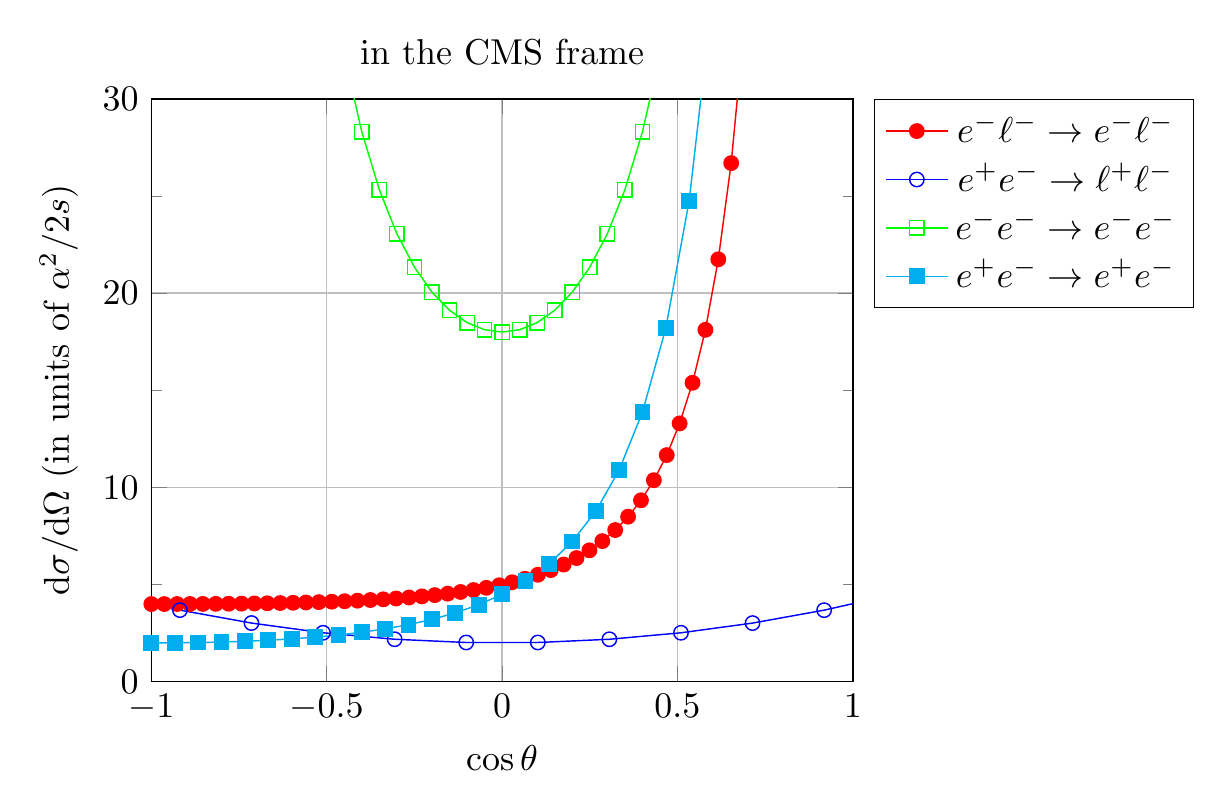
\begin{tikzpicture}[scale=1.3]
    \begin{axis}[
        title=in the CMS frame,
        xlabel={$\cos\theta$},
        ylabel={$\d\sigma/\d\Omega$ (in units of $\alpha^2/2s$)},
        xmin=-1, xmax=1,
        ymin = 0, ymax=30,
        minor y tick num=1,
        grid = major,
        legend entries={$e^-\ell^-\rightarrow e^-\ell^-$,
        $e^+e^-\rightarrow \ell^+\ell^-$,
        $e^-e^-\rightarrow e^-e^-$,
        $e^+e^-\rightarrow e^+e^-$
        },
        legend style={legend pos = outer north east}
    ]
        \addplot [red,samples=50,domain=-1:0.8, mark=*] {(4+(1+x)^2/(1-x)^2))};
        \addplot [samples=50,blue, mark=o] {2*(1+x^2)};
        \addplot [green,domain=-0.6:0.6, mark=square] {(4+(1+x)^2)/(1-x)^2+((4+(1-x)^2)/(1+x)^2)+8/(1-x^2)};
        \addplot [cyan,domain=-1:0.6, mark=square*] {(3+x^2)^2/(2*(x-1)^2};
   \end{axis}
\end{tikzpicture}%
\caption{Angular dependencies in the center-of-mass frame
of the differential cross-sections
for the main QED processes. The label $\ell$ stands for either muon or tau.}
\end{center}
\end{figure}
%%%%%%%%%%%%%%%%% END FIGURE %%%%%%%%%%%%%%%%%%%%%%%%%%%%%%
%

\end{document}
